\let\negmedspace\undefined
\let\negthickspace\undefined
\documentclass[journal,12pt,twocolumn]{IEEEtran}

\usepackage{cite}
\usepackage{amsmath,amssymb,amsfonts,amsthm}
\usepackage{algorithmic}
\usepackage{graphicx}
\usepackage{textcomp}
\usepackage{xcolor}
\usepackage{txfonts}
\usepackage{listings}
\usepackage{enumitem}
\usepackage{mathtools}
\usepackage{gensymb}
\usepackage[breaklinks=true]{hyperref}
\usepackage{tkz-euclide} % loads  TikZ and tkz-base
\usepackage{listings}
\usepackage{circuitikz}
\usepackage{graphicx}

%\newcounter{MYtempeqncnt}
\DeclareMathOperator*{\Res}{Res}
%\renewcommand{\baselinestretch}{2}
\renewcommand\thesection{\arabic{section}}
\renewcommand\thesubsection{\thesection.\arabic{subsection}}
\renewcommand\thesubsubsection{\thesubsection.\arabic{subsubsection}}

\renewcommand\thesectiondis{\arabic{section}}
\renewcommand\thesubsectiondis{\thesectiondis.\arabic{subsection}}
\renewcommand\thesubsubsectiondis{\thesubsectiondis.\arabic{subsubsection}}

% correct bad hyphenation here
\hyphenation{op-tical net-works semi-conduc-tor}
\def\inputGnumericTable{}                                 %%

\lstset{
	frame=single,
	breaklines=true,
	columns=fullflexible
}

\newtheorem{theorem}{Theorem}[section]
\newtheorem{problem}{Problem}
\newtheorem{proposition}{Proposition}[section]
\newtheorem{lemma}{Lemma}[section]
\newtheorem{corollary}[theorem]{Corollary}
\newtheorem{example}{Example}[section]
\newtheorem{definition}[problem]{Definition}
\newcommand{\BEQA}{\begin{eqnarray}}
	\newcommand{\EEQA}{\end{eqnarray}}
\newcommand{\define}{\stackrel{\triangle}{=}}
\newcommand\figref{Fig.~\ref}
\newcommand\tabref{Table~\ref}
\bibliographystyle{IEEEtran}
%\bibliographystyle{ieeetr}


\providecommand{\mbf}{\mathbf}
\providecommand{\pr}[1]{\ensuremath{\Pr\left(#1\right)}}
\providecommand{\qfunc}[1]{\ensuremath{Q\left(#1\right)}}
\providecommand{\sbrak}[1]{\ensuremath{{}\left[#1\right]}}
\providecommand{\lsbrak}[1]{\ensuremath{{}\left[#1\right.}}
\providecommand{\rsbrak}[1]{\ensuremath{{}\left.#1\right]}}
\providecommand{\brak}[1]{\ensuremath{\left(#1\right)}}
\providecommand{\lbrak}[1]{\ensuremath{\left(#1\right.}}
\providecommand{\rbrak}[1]{\ensuremath{\left.#1\right)}}
\providecommand{\cbrak}[1]{\ensuremath{\left\{#1\right\}}}
\providecommand{\lcbrak}[1]{\ensuremath{\left\{#1\right.}}
\providecommand{\rcbrak}[1]{\ensuremath{\left.#1\right\}}}
\theoremstyle{remark}
\newtheorem{rem}{Remark}
\newcommand{\sgn}{\mathop{\mathrm{sgn}}}
\providecommand{\abs}[1]{\left\vert#1\right\vert}
\providecommand{\res}[1]{\Res\displaylimits_{#1}}
\providecommand{\norm}[1]{\left\lVert#1\right\rVert}
%\providecommand{\norm}[1]{\lVert#1\rVert}
\providecommand{\mtx}[1]{\mathbf{#1}}
\providecommand{\mean}[1]{E\left[ #1 \right]}
\providecommand{\fourier}{\overset{\mathcal{F}}{ \rightleftharpoons}}
%\providecommand{\hilbert}{\overset{\mathcal{H}}{ \rightleftharpoons}}
\providecommand{\system}{\overset{\mathcal{H}}{ \longleftrightarrow}}
%\newcommand{\solution}[2]{\textbf{Solution:}{#1}}
\newcommand{\solution}{\noindent \textbf{Solution: }}
\newcommand{\cosec}{\,\text{cosec}\,}
\providecommand{\dec}[2]{\ensuremath{\overset{#1}{\underset{#2}{\gtrless}}}}
\newcommand{\myvec}[1]{\ensuremath{\begin{pmatrix}#1\end{pmatrix}}}
\newcommand{\mydet}[1]{\ensuremath{\begin{vmatrix}#1\end{vmatrix}}}
\renewcommand{\abstractname}{Question}

\let\vec\mathbf

\vspace{3cm}
	

\newcommand{\permcomb}[4][0mu]{{{}^{#3}\mkern#1#2_{#4}}}
\newcommand{\comb}[1][-1mu]{\permcomb[#1]{C}}

%\IEEEpeerreviewmaketitle

\newcommand \tab [1][1cm]{\hspace*{#1}}
%\newcommand{\Var}{$\sigma ^2$}
\usepackage{amssymb}
\usepackage{amsmath}
\title{
	
\title{NCERT Physics 12.7 Q19}
\author{EE23BTECH11212 - MANUGUNTA MEGHANA SAI$^{*}$% <-this % stops a space
}


}
\begin{document}

\maketitle

\textbf{Question:} 
Suppose the circuit in Exercise 7.18 (in Figure~\figref{fig:2})has a resistance of 15 Ω. Obtain the average power transferred to each element of the circuit, and the total power absorbed.\\
\\

\begin{figure}[h]
	\centering
	    %\begin{circuitikz}
		% Draw the components
	%	\draw (0,0) to[V, v=$230\,V$, f=$50\,Hz$] (0,3)
	%	to[R, l=$15\,\Omega$] (3,3)
	%	to[L, l=$80\,mH$] (6,3)
	%	to[C, l=$60\,\mu F$] (6,0)
	%	-- (0,0);
    % \end{circuitikz}
\begin{circuitikz}
	\draw(0, 0) -- (1, 0);
	\draw(1, 0) to [L, l = $80\,mH$](2, 0);
	\draw(2, 0) -- (3, 0);
	\draw(3, 0) to [C, l = $60\,\mu F$](4, 0);
	\draw(4, 0) -- (5, 0);
	\draw(5, 0) to [R, l = $15\,\Omega$](6, 0);
	\draw(0, 0) -- (0, -2);
	\draw[->] (0, -1) node[left] {$I(s)$} -- (0, -1);
	\draw(6, 0) -- (7, 0);
	\draw(7, 0) -- (7, -2);
	\draw(0, -2) -- (3, -2);
	\draw(7, -2) -- (7, -2);
	\draw(3, -2) to [sV, l = $230\,V$](4, -2);
	\draw(4, -2) -- (7, -2);
\end{circuitikz}


	\caption{LCR Circuit}
	\label{fig:2}
\end{figure}
     
\textbf{Solution: }
In~\figref{fig:2} the following information is provided:
 
 

 \begin{table}[h]
 	\centering
 	\resizebox{6 cm}{!}{
 		\begin{tabular}{|c|c|c|}
	\hline
	\textbf{Symbol} & \textbf{Value} &
	\textbf{Description}\\[6pt]
	\hline
	L &  $80m\,
	\text{H}$ & Inductance\\[6pt]
	\hline 
	C &  $60\, \mu\text{F}$ & Capacitance \\[6pt]
	\hline
	R &  $15\, \Omega$ & Resistance\\[6pt]
	\hline
	V & $230\, \text{V}$ & Voltage\\[6pt]
	\hline
	f & $50\, \text{Hz}$ & Frequency\\[6pt]
	\hline
\end{tabular}
 	}
 	\vspace{6 pt}
 	\caption{Given Parameters}
 	\label{tab:my_label} 
 \end{table} 
 \text{Applying Kirchoff's Voltage Law} in the~\figref{fig:1}
 
 \begin{figure}[!h]
 	\centering
 	\begin{circuitikz}
	\draw(0, 0) -- (1, 0);
	\draw(1, 0) to [L, l = $sL$](2, 0);
	\draw(2, 0) -- (3, 0);
	\draw(3, 0) to [C, l = $\frac{1}{sC}$](4, 0);
	\draw(4, 0) -- (5, 0);
	\draw(5, 0) to [R, l = $R$](6, 0);
	\draw(0, 0) -- (0, -2);
	\draw[->] (0, -1) node[left] {$I(s)$} -- (0, -1);
	\draw(6, 0) -- (7, 0);
	\draw(7, 0) -- (7, -2);
	\draw(0, -2) -- (3, -2);
	\draw(7, -2) -- (7, -2);
	\draw(3, -2) to [sV, l = $V(s)$](4, -2);
	\draw(4, -2) -- (7, -2);
\end{circuitikz}
 	\caption{s domain circuit}
 	\label{fig:1}
 	
 \end{figure}
 \begin{align}
 	V(s) &= R I(s) + sL I(s) + \dfrac{1}{sC} I(s)\\
         &= I(s)\left(R + Ls + \dfrac{1}{sC}\right)
 \end{align}
\begin{align}
    I(s) &= \dfrac{V(s)}{\left(R + Ls + \dfrac{1}{sC}\right)}\\ 
    H(s) &= \dfrac{V(s)}{I(s)}\\
	H(s) &= R + sL + \dfrac{1}{sC}
\end{align}

Substituting $s$ with $\j \omega$
\begin{equation}
	H(j\omega) = R + j\omega L + \dfrac{1}{j\omega C}
\end{equation}
\begin{equation}
	\Rightarrow \lvert H(j\omega) \rvert = \sqrt{R^2 + \left(\omega L - \dfrac{1}{\omega C}\right)^2}
	\label{eq:1}
\end{equation}
Average power transferred to an element in the circuit is given by:
\begin{align}
	P=VIcos(\phi) 
\end{align}

a) Average power transferred to the capacitor, $P_C$:
For a capacitor the phase angle is:
\begin{align}
	\phi &= \frac{\pi}{2}\\
	cos(\phi) &= 0\\
	P_C &= 0
\end{align}	  
b) Average power transferred to the inductor, $P_L$:
For an inductor the phase angle is:
\begin{align}
	\phi &= -\frac{\pi}{2}\\
	cos(\phi) &= 0\\
	P_L &= 0
\end{align}	 

c) Average Power transferred to the resistor, $P_R$:
$|H(j\omega)|$ is obtained by sustituting the numerical values from the ~\tabref{tab:my_label} in equation (~\ref{eq:1}):
\begin{align}
	|H(j\omega)|=31.728\hspace{0.2cm}\ohm
\end{align}	

\begin{align}
	I_{rms}=\frac{V_{rms}}{H(j\omega)}=\frac{230}{31.728}=7.25A
\end{align}
\begin{align}
	P_R=(I_{rms})^2R = 788.44W
\end{align}

d)Total power absorbed by circuit:

\begin{align}
	&= P_R + P_C + P_L
	\\&= 788.44 + 0 + 0
	\\&= 788.44\hspace{0.2cm}W
\end{align}

Total power absorbed by circuit is 788.44\hspace{0.01cm}W
\vspace{1cm}
\begin{figure}[h!]
	\centering
	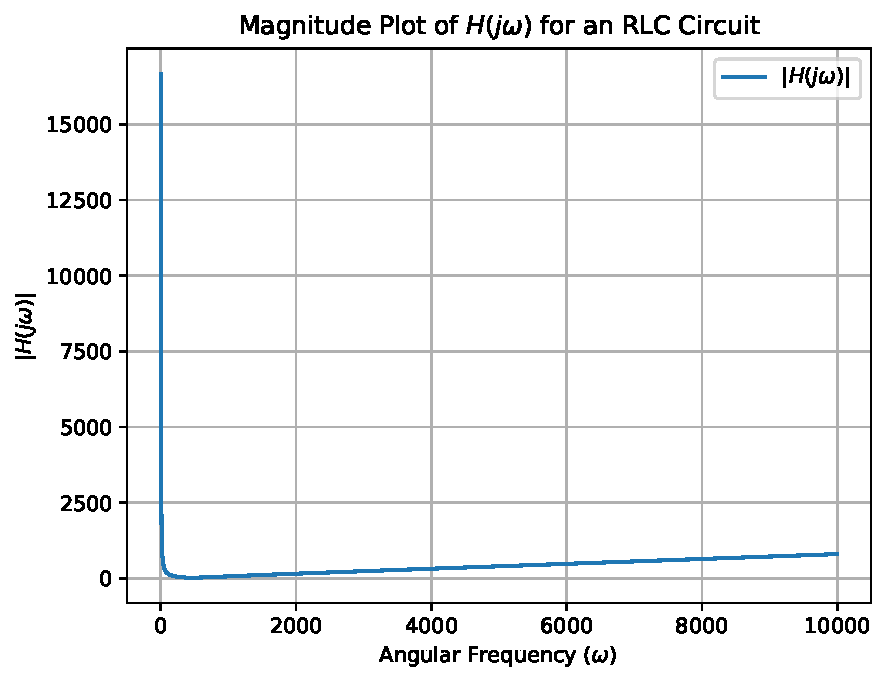
\includegraphics[width=\columnwidth]{figs/garph1.pdf}
	\caption{$|H(j/omega)|$ vs $\omega$}
	\label{fig:magnitude_plot}
\end{figure}
\end{document}

